\documentclass[
	% -- opções da classe memoir --
	12pt,				% tamanho da fonte
	openright,			% capítulos começam em pág ímpar (insere página vazia caso preciso)
	oneside,			% para impressão em verso e anverso. Oposto a oneside
	a4paper,			% tamanho do papel. 
	% -- opções do pacote babel --
	% idioma adicional para hifenização
	brazil,				% o último idioma é o principal do documento
	]{abntex2}


\usepackage{cmap}				% Mapear caracteres especiais no PDF
\usepackage{lmodern}			% Usa a fonte Latin Modern			
\usepackage[T1]{fontenc}		% Selecao de codigos de fonte.
\usepackage[utf8]{inputenc}		% Codificacao do documento (conversão automática dos acentos)
\usepackage{lastpage}			% Usado pela Ficha catalográfica
\usepackage{indentfirst}		% Indenta o primeiro parágrafo de cada seção.
\usepackage{color}				% Controle das cores
\usepackage{graphicx}			% Inclusão de gráficos
\usepackage{amsmath}
\usepackage{mathtools}

\usepackage[brazilian,hyperpageref]{backref}	 % Paginas com as citações na bibl
\usepackage[alf]{abntex2cite}	% Citações padrão ABNT

\usepackage{algorithm}
\usepackage[noend]{algpseudocode}
\usepackage{amsfonts}

\makeatletter
\def\BState{\State\hskip-\ALG@thistlm}
\makeatother

\usepackage{caption}
\usepackage{subcaption}
\usepackage{hyperref}
\hypersetup{
    colorlinks=true,
    linkcolor=blue,
    filecolor=magenta,      
    urlcolor=cyan,
}
 
\urlstyle{same}


% Incluir código fonte
\usepackage{minted}

% Use wide margins, but not quite so wide as fullpage.sty
\marginparwidth 0.5in 
\oddsidemargin 0.25in 
\evensidemargin 0.25in 
\marginparsep 0.25in
\topmargin 0.25in 
\textwidth 6in \textheight 8 in
% That's about enough definitions

% multirow allows you to combine rows in columns
\usepackage{multirow}
% tabularx allows manual tweaking of column width
\usepackage{tabularx}
% longtable does better format for tables that span pages
\usepackage{longtable}




\titulo{Desviando de obstaculos com fuzzy e aprendizagem por reforço}
\author{Samuel Cavalcanti\\}
\orientador{Professor: Sérgio Natan Silva}
\instituicao{%
  Universidade Federal do Rio Grande do Norte
  \par
  Centro de Tecnologia
  \par
  Departamento de Computação e Automação
  \par
  Engenharia de Computação}

\local{Natal}
\date{14 de junho de 2019 }



% ---
% Configurações de aparência do PDF final

% informações do PDF
\makeatletter
\hypersetup{
     	%pagebackref=true,
		pdftitle={\@title}, 
		pdfauthor={\@author},
    	pdfsubject={\imprimirpreambulo},
	    pdfcreator={LaTeX with abnTeX2},
		pdfkeywords={abnt}{latex}{abntex}{abntex2}{trabalho acadêmico}, 
		colorlinks=true,       		% false: boxed links; true: colored links
    	linkcolor=black,          	% color of internal links
    	citecolor=black,        		% color of links to bibliography
    	filecolor=black,      		% color of file links
		urlcolor=black,
		bookmarksdepth=4
}
\makeatother
% --- 

% --- 
% Espaçamentos entre linhas e parágrafos 
% --- 

% O tamanho do parágrafo é dado por:
\setlength{\parindent}{1.3cm}

% Controle do espaçamento entre um parágrafo e outro:
\setlength{\parskip}{0.2cm}  % tente também \onelineskip

% ---
% compila o indice
% ---
\makeindex
% ---

% ----
% Início do documento
% ----
\begin{document}

% Retira espaço extra obsoleto entre as frases.
\frenchspacing 

% ----------------------------------------------------------
% ELEMENTOS PRÉ-TEXTUAIS
% ----------------------------------------------------------
% ---
% Capa
% ---
\imprimircapa
% ---

% ---
% inserir o sumario
% ---
\pdfbookmark[0]{\contentsname}{toc}
\tableofcontents*
\cleardoublepage
% ---



% ----------------------------------------------------------
% ELEMENTOS TEXTUAIS
% ----------------------------------------------------------
\textual

% ----------------------------------------------------------
% Introdução
% ----------------------------------------------------------
\chapter{Introdução}
Recentemente navegação de robôs moveis tem se tornado um grande objeto de estudo dentro da robótica e no campo da inteligência artificial. O problema da navegação robótica é  o robô escolher a decisão correta de conseguir completar a tarefa de encontrar o seu destino sem colidir com obstáculos, de acordo com a informação do ambiente captada pelos sensores \cite{duan2005fuzzy}.

Aprendizagem por reforço é uma técnica de aprendizagem de máquina que aprende com a interação com o ambiente. Duas de suas principais características comparada outras técnicas de aprendizagem de máquina é busca por tentativa e erro e sua recompensa atrasada \cite{sutton2018reinforcement}. A busca é realizada a medida que o agente interage com o ambiente e após uma ação ou um conjunto delas o agente recebe uma recompensa. A aprendizagem por reforço é recomendada quando não se é possível obter bons exemplos para todas as situações. Então nesses casos o agente tem que aprender pela própria experiência \cite{zhangreinforcement}.

Um dos grandes desafios do aprendizado por reforço é o gerenciamento do quanto o agente deve tentar ações ainda não conhecidas e quando ele vai executar ações que maximiza a sua recompensa. Para resolver esse desafio além do agente contar com o próprio conhecimento, foi utilizado aprendizagem por demonstração.Com a aprendizagem por demonstração uma sequência de estado-ação é aprendido a partir de um exemplo ensinado por um professor. Um exemplo é um comportamento, uma sequência de estado-ação que foi gravado durante a demonstração do professor \cite{argall2009survey}. 

Outro desafio da aprendizagem por reforço é a definição da função recompensa, uma vez que os algoritmos visam maximizar essa função o que não necessariamente ira gerar o comportamento desejado. Abordagem utilizada para gerar a função recompensa foi a logica nebulosa. A teoria dos conjuntos nebulosos, quando utilizada em um contexto lógico, como o de sistemas baseados em conhecimento, é conhecida como lógica nebulosa, lógica difusa ou lógica “fuzzy”\cite{sandri1999logica}. Um controlador logico fuzzy é um sistema especialista baseado em regras de se-então, que busca representar a linguagem natural humana \cite{duan2005fuzzy}.

Esse relato está contextualizado no problema de navegação de robôs moveis utilizado técnicas de aprendizagem por reforço para encontrar a melhor politica ou estado-ação para desviar de obstáculos. Onde a função de reforço é dada por um controlador logico fuzzy e para reduzir o tempo de aprendizagem, foi feito uma única demonstração para o robô de uma possível política que ele poderia seguir para desviar de obstáculos. A utilização de aprendizagem por reforço e controlador logico fuzzy para resolver esse problema não é novidade, um sistema utilizando essas duas técnicas já foi proposto por \cite{duan2005fuzzy}, onde ele utilizou uma Q($\gamma$)-learning e um controlador fuzzy, para resolver esse problema. A utilização de aprendizagem por demonstração também não é novidade , onde  \cite{argall2009survey} utilizou aprendizagem pro demonstração para ensinar uma política a um robô.


\chapter{Abordagem Teórica}\label{Teoria}

Nesse relato foi utilizado um robô simulado, implementado o deep Q-learning com algumas alterações necessárias para o problema com a biblioteca keras e criado a função de recompensa com a biblioteca skfuzzy.
 


\section{aprendizado por reforço}
Aprendizado por reforço é o aprendizado de como mapear situações para ações de modo que maximize uma função recompensa. O aprendiz não sabe a priore quais ações deve realizar, ele deve descobrir quais ações maximizam a função recompensa a partir da tentativa e erro. O fato mais interessante é que as ações não só afetam a recompensa imediata como também afetam a recompensa das próximas situações. Aprendizado por reforço é um conjunto de soluções que visam resolver problemas oriundos da teoria de sistemas dinâmicos e otimização de controle de processos markovianos \cite{sutton2018reinforcement}. dentre esse conjunto de soluções o algoritmo deep Q-learning with experience replay foi escolhido \ref{DQNN}. O deep Q network (DQN) é uma rede neural de múltiplas camadas que recebe um estado $s$ e lhe dá como saída um vetor de ações $Q(s, \cdot ;\theta)$ , onde $\theta$ são os parâmetros da rede. Para um espaço $n-$dimensional e o espaço $m$ de ações. A rede neural é uma função do  $\mathbb{R}^n$ para $\mathbb{R}^m$. Dois importantes passos desse algoritmo proposto por \cite{mnih2015human} foi o uso do rede alvo e uma adaptação chamada de memória ou experience replay. Rede alvo é usar a própria saída da rede como parte do vetor de amostras com a diferença que o nodo vencedor será atualizado seguindo a equação \ref{target_DQN}.

\begin{equation}\label{target_DQN}
 y^{DQN}_j = r_j + \gamma\textrm{argmax}_{\acute{a}}\hat{Q}(\theta_{j+1},\acute{a};\bar{\theta})
\end{equation}

Já a memória é uma estrutura onde é armazenado por um determinado período de tempo as transições observadas pelo agente. A partir desse banco de memórias é que a rede neural será atualizada. Tanto a rede alvo quando o a memória melhoram a performance do algoritmo \cite{van2016deep} , \cite{mnih2015human}

O algoritmo de aprendizado por reforço usado foi o deep Q-learning com o uso da memória \cite{mnih2015human}. O seu pseudo código pode ser encontrado aqui \ref{DQNN}

\begin{algorithm}[H]
\caption{deep Q-learning with experience replay}\label{DQNN}
\begin{algorithmic}[1]
\State inicialize a memoria D com capacidade N
\State inicialize a função ação-valor Q com pesos randômicos $\theta$
\State inicialize a função de valor de destino $\hat{Q}$ com pesos $\bar{\theta} = 0$
 \For  {episódio =1, M}
\State $s_t =$ valores dos sensores
\State Com probabilidade  $\epsilon$ selecione uma ação randômica $a_t$
\State ou selecione $a_t = \textrm{argmax}_a Q((s_t),a;\theta)$
\State Execute a  ação  $a_t$ no simulador e observe a recompensa $r_t$ e o estado $s_{t+1}$
\State armazene a transição ($s_j$,$a_j$,$r_j$,$s_{j+1}$) em D
\State recupere um mine pacote de amostras de transições ($s_t$,$a_t$,$r_t$,$s_{t+1}$) de D
\If {o episódio acabar no passo $j+1$}
\State $y_j = r_j$
\Else
\State $y_j = r_j + \gamma\textrm{argmax}_{\acute{a}}\hat{Q}(\theta_{j+1},\acute{a};\bar{\theta}) $
\EndIf
\State Use o gradiente descendente em $(y_j - Q(s_j,a_j;\theta))^2 $ no parâmetros $\theta$ da rede neural
\EndFor
\end{algorithmic}
\end{algorithm}

\section{Controlador logico nebuloso}
As técnicas de controle nebuloso originaram-se comas pesquisas e projetos de \cite{mamdani1976advances} ,\cite{mamdani1976application}  e ganharam espaço como área de estudo em diversas instituições de ensino, pesquisa e desenvolvimento do mundo, sendo até hoje uma importante aplicação da teoria dos conjuntos nebulosos.Ao contrário dos controladores convencionais em que o algoritmo de controle é descrito analiticamente por equações algébricas ou diferenciais, através de um modelo matemático, em controle nebuloso utilizam-se de regras lógicas no algoritmo de controle, com a intenção de descrever numa rotina a experiência humana, intuição e heurística para controlar um processo \cite{sandri1999logica}.

\section{aprendizagem por demonstração}
O princípio de aprendizagem por demonstração ( learning from demonstration- LfD) se baseia em ensinar novas tarefas a robôs sem a necessidade de programação. Tomando em conta um cenário clássico de programação, se faz necessário primeiramente programar todas as tarefas que se deseja que o robô realize, sendo necessário cobrir todas as possibilidades e adversidades que possam ocorrer nesse cenário. Esse processo porém, envolve muitas etapas e testes, e caso erros ou novas circunstâncias ocorram depois da implementação no robô, muitas e em alguns casos todas as etapas do processo precisam ser refeita \cite{ekvall2008robot}.Técnicas e métodos de aprendizagem por demonstração permitem ao usuário final comandar e especificar tarefas a serem realizadas pelo robô, sem nenhuma necessidade de programação, apenas demonstrando fisicamente como realizá-las. Dessa forma, quando algum erro ou adversidade ocorrer, será necessário apenas fornecer mais demonstrações para o robô, evitando assim a necessidade de reprogramação do mesmo. \cite{motta2016aprendizagem}.


\chapter{Descrição da Proposta}\label{Descricao}
Para avaliar o sistema que desvia de obstáculos, foi feito uma simulação que a partir dela foi observado os valores do sensores para a formação das regras do controlador fuzzy. Por ultimo criado uma estratégia de treinamento envolvendo aprendizagem por demonstração. Para facilitar o leitor esse capítulo foi dividido em 3 partes: a primeira irá detalhar a simulação, a segunda será sobre o controlador fuzzy e a ultima contará a estratégia de treinamento. 

\section{Simulação}
O simulador utilizado foi o V-rep. Um simulador de robótica que provê uma quantidade razoável de robôs já prontos e boa documentação. A partir desse simulador foi selecionado o robô Pioneer \ref{Pioneer} a qual possui dezesseis sensores ultrassônicos e tração diferencial \ref{Pioneer_sensors}. Como o número de regras cresce exponencialmente com o número de entradas do controlador fuzzy. Foi então decidido limitar o movimentação do robô para frente e para a esquerda e retirar doze sensores para simplificar o problema. Nesse relato foi utilizado duas cenas, a primeira \ref{scene_1} é a mais simples utilizada para treinamento do algoritmo, é um único cômodo fechado a quatro paredes, a segunda \ref{scene_2} , simula um apartamento com três cômodos e um corredor, essa cena foi utilizada para avaliar o sistema de controle.

\begin{figure}[h]
\centering
	\begin{subfigure}{.5\textwidth}
		\centering
   		 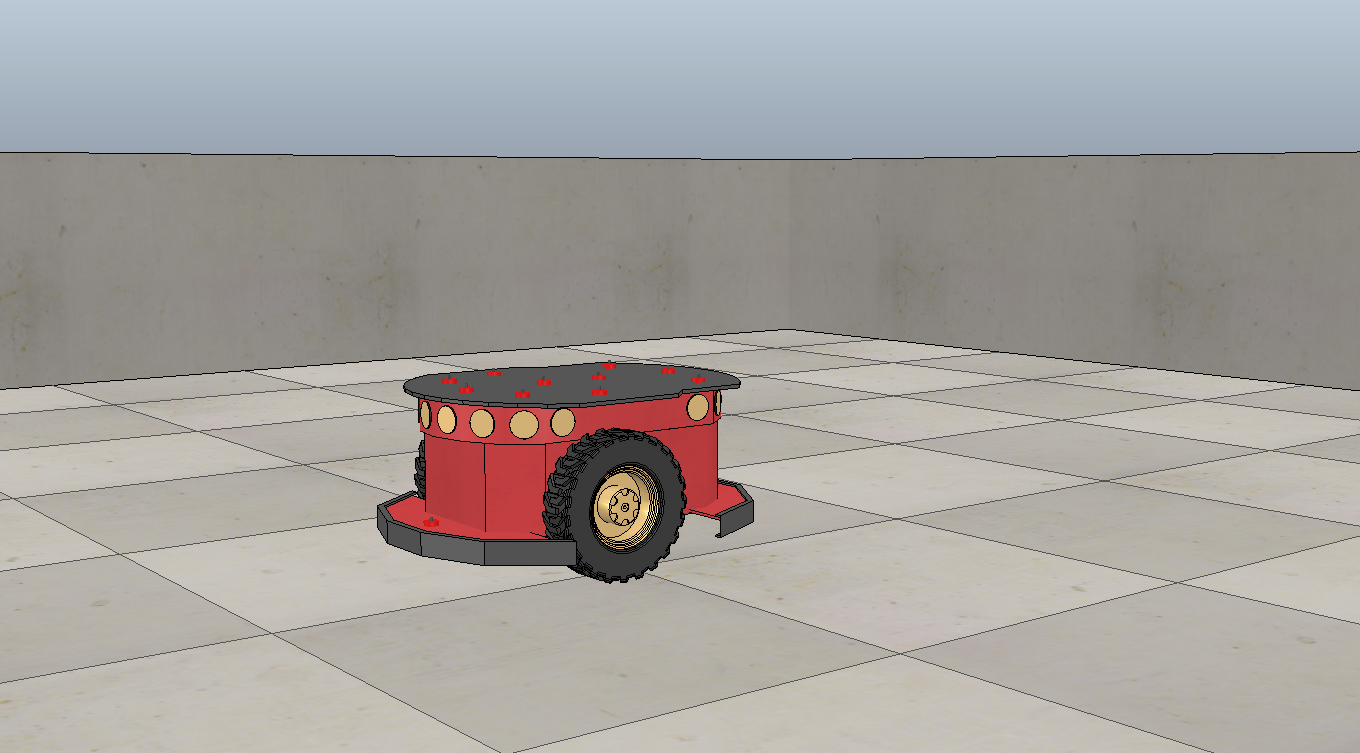
\includegraphics[width = 0.4\textwidth]{Imagens/Pioneer.png}
    	 \caption{Robô Pioneer}
   		 \label{Pioneer}
    \end{subfigure}%
    \begin{subfigure}{.5\textwidth}
		\centering
   		 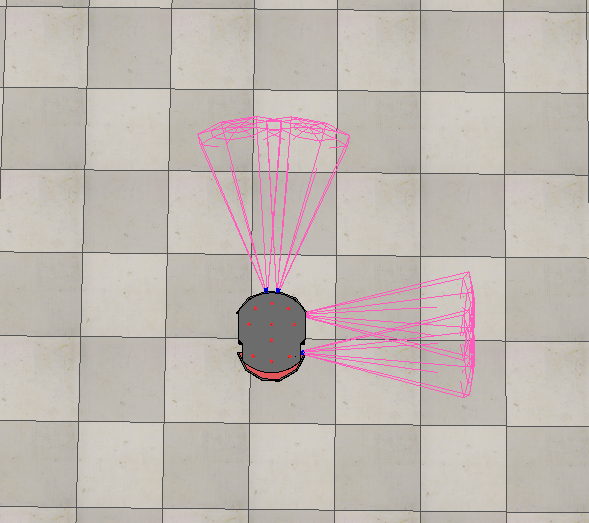
\includegraphics[width = 0.4\textwidth]{Imagens/Pioneer_sensors.png}
    	 \caption{ sensores do Pioneer}
   		 \label{Pioneer_sensors}
    \end{subfigure}
    
    \begin{subfigure}{.5\textwidth}
		\centering
   		 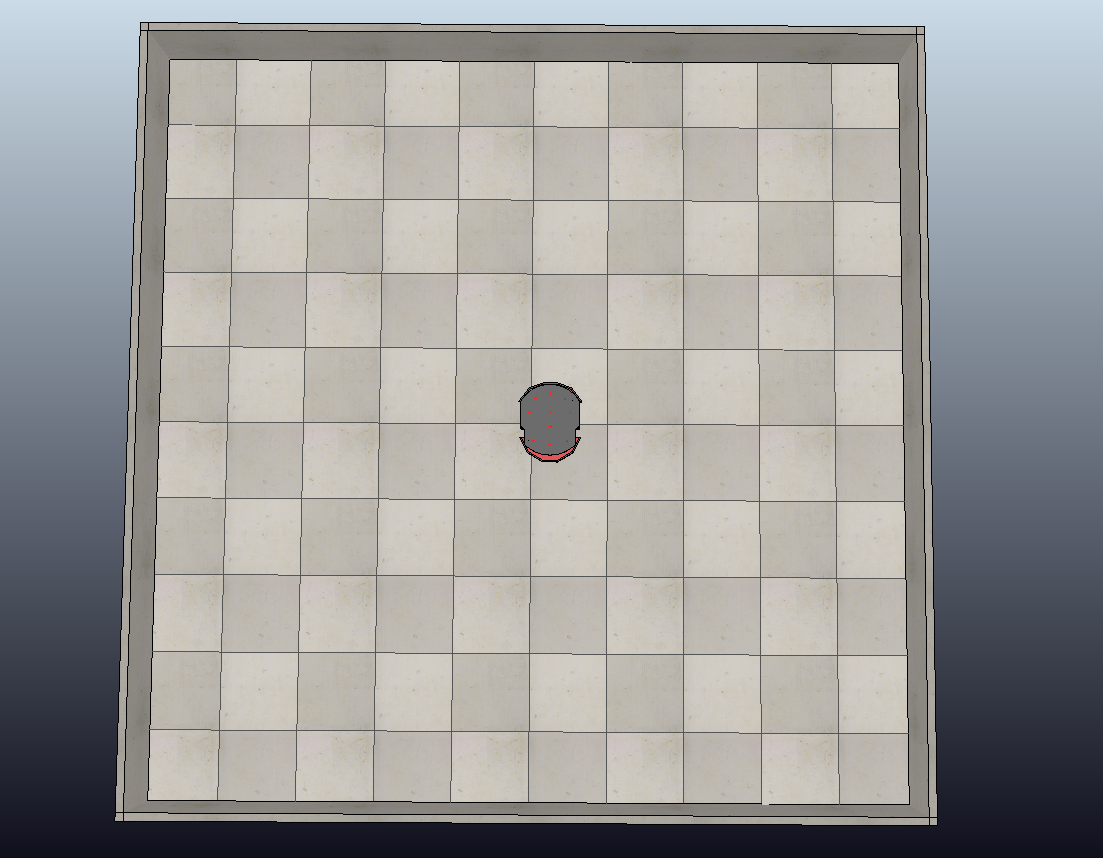
\includegraphics[width = 0.4\textwidth]{Imagens/scene_1.png}
    	 \caption{cena de treinamento}
   		 \label{scene_1}
    \end{subfigure}%
    \begin{subfigure}{.5\textwidth}
		\centering
   		 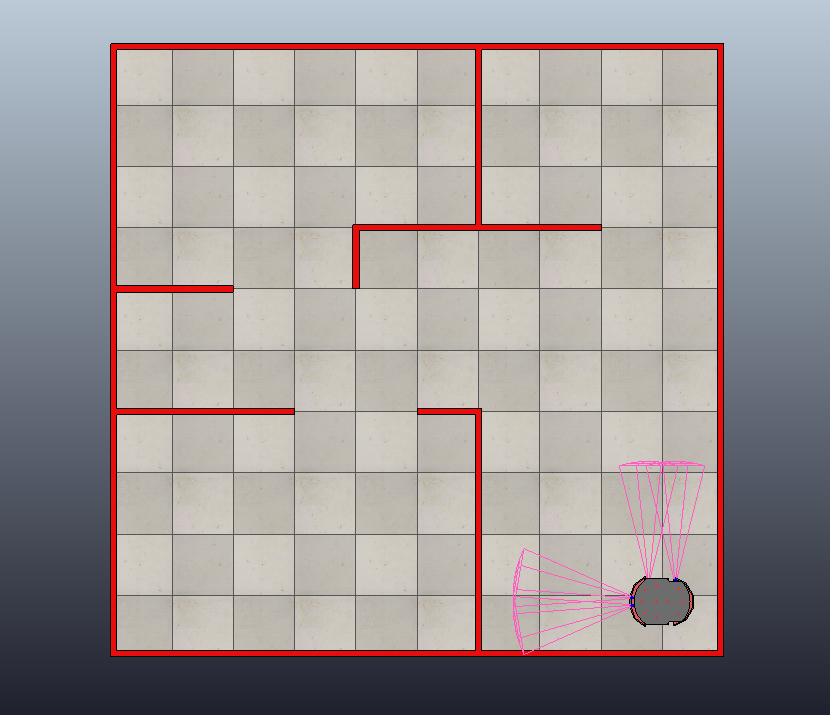
\includegraphics[width = 0.4\textwidth]{Imagens/scene_2.png}
    	 \caption{ cena de validação}
   		 \label{scene_2}
    \end{subfigure}
    
\end{figure}


\section{Controlador fuzzy}
O controlador fuzzy funcionava como uma função que recebe a média dos sensores da frente e a média dos sensores da direita como entrada, e retornava um valor entre menos um e um. Para chegar nessa função foi necessário duas logicas fuzzy, a primeira mensurava o quão distante estava uma das media dos sensores  até o obstáculo ,a segunda mensurava a recompensa a partir  da primeira. A primeira logica transformava a distancia das médias dos sensores em um grau de pertinência de trés classes: perto, bom , longe. A classe perto é um trapézio definido nos pontos: $(-1,2,0,0.2,0.3)$, a classe bom é um triangulo com os pontos: $(0.2, 0.4, 0.7)$e a classe longe é outro trapézio com os pontos $(0.6, 0.8, 1, 1.2)$. Ambas as médias dos sensores passam por essa mesma lógica que pode ser melhor compreendida no gráfico \ref{sensor}. Para a segunda lógica foi necessário criar cinco regras que mapeasse o grau de pertinência de cada classe para trés tipos recompensa: ruim, neutra e boa. As cinco regras foram:
\begin{itemize}
	\item \textbf{Se} a média dos sensores da frente \textbf{OU} a média dos sensores da direita for perto \textbf{então} a recompensa é ruim
	\item \textbf{Se} a média dos sensores da frente for boa \textbf{\&} a média dos sensores da direita for boa \textbf{então} a recompensa é boa 
	\item \textbf{Se} a média dos sensores da frente for boa \textbf{\&} a média dos sensores da direita for longe \textbf{então} a recompensa é boa 
	\item \textbf{Se} a média dos sensores da frente for longe \textbf{\&} a média dos sensores da direita for boa \textbf{então} a recompensa é boa 
\	\item \textbf{Se} a média dos sensores da frente for longe \textbf{\&} a média dos sensores da direita for longe \textbf{então} a recompensa é neutra
\end{itemize}
Depois das regras foi definido o formato da função de cada classe da logica da recompensa. A classe ruim é um triangulo com os pontos: $(-1, -1, 0)$ , classe neutra é um triangulo com os pontos: $(-0.5, 0, 0.5)$ e a classe boa é um triangulo com os pontos: $(0, 1, 1.2)$ essa funções podem ser melhor compreendida no gráfico \ref{reward}, \ref{surface_control}, \ref{surface_control2}. O processo de defuzzificação utilizado é o centroide.

\begin{figure}[H]
	\centering
	 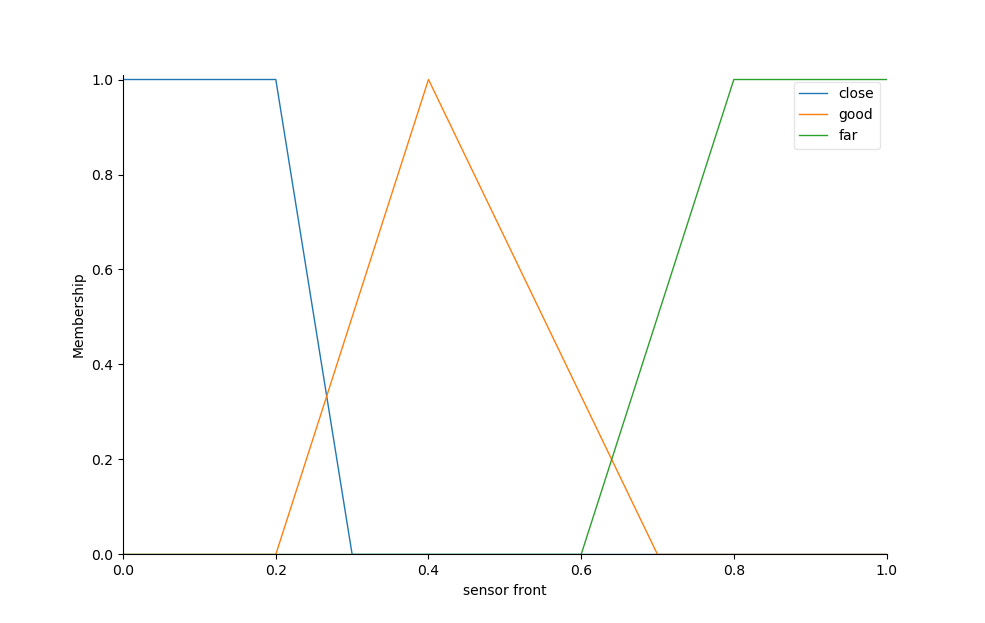
\includegraphics[width = 1\textwidth]{Imagens/sensor.png}
	 \caption{logica fuzzy da distancia de um sensor até o obstáculo}
	 \label{sensor}
	
	 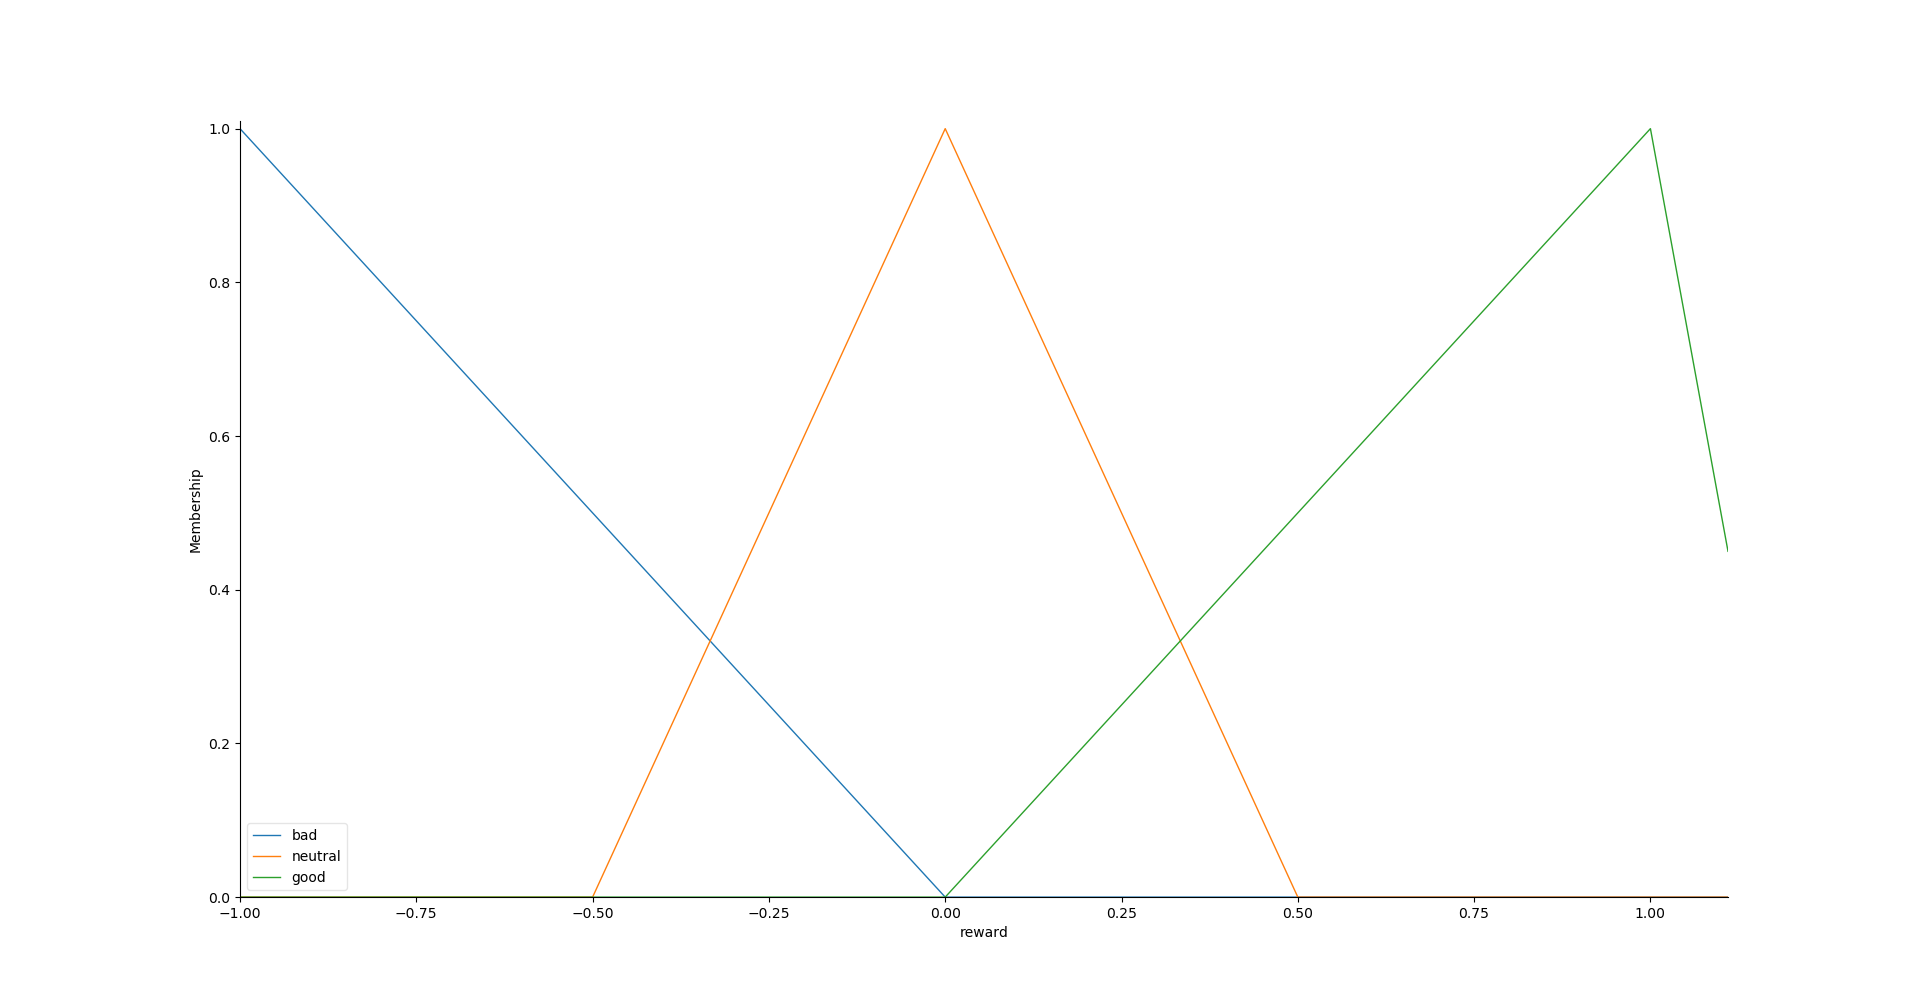
\includegraphics[width = 1\textwidth]{Imagens/reward.png}
	 \caption{logica fuzzy da recompensa}
	 \label{reward}
	 
\end{figure}%
%
\begin{figure}[H]
 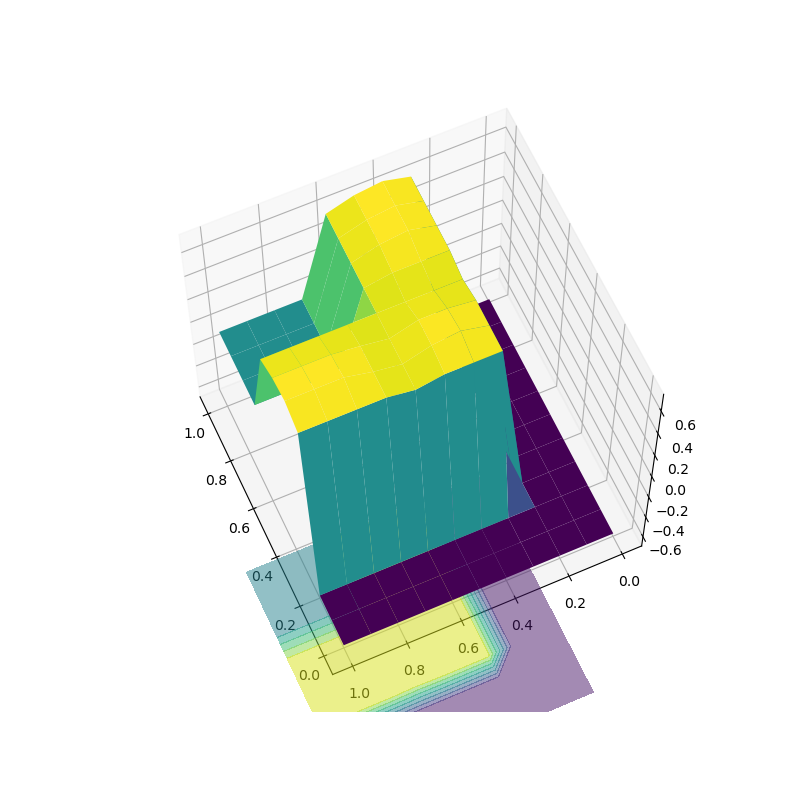
\includegraphics[width = 1\textwidth]{Imagens/Surface_Control.png}
	 \caption{superfície de controle}
	 \label{surface_control}
	 
	 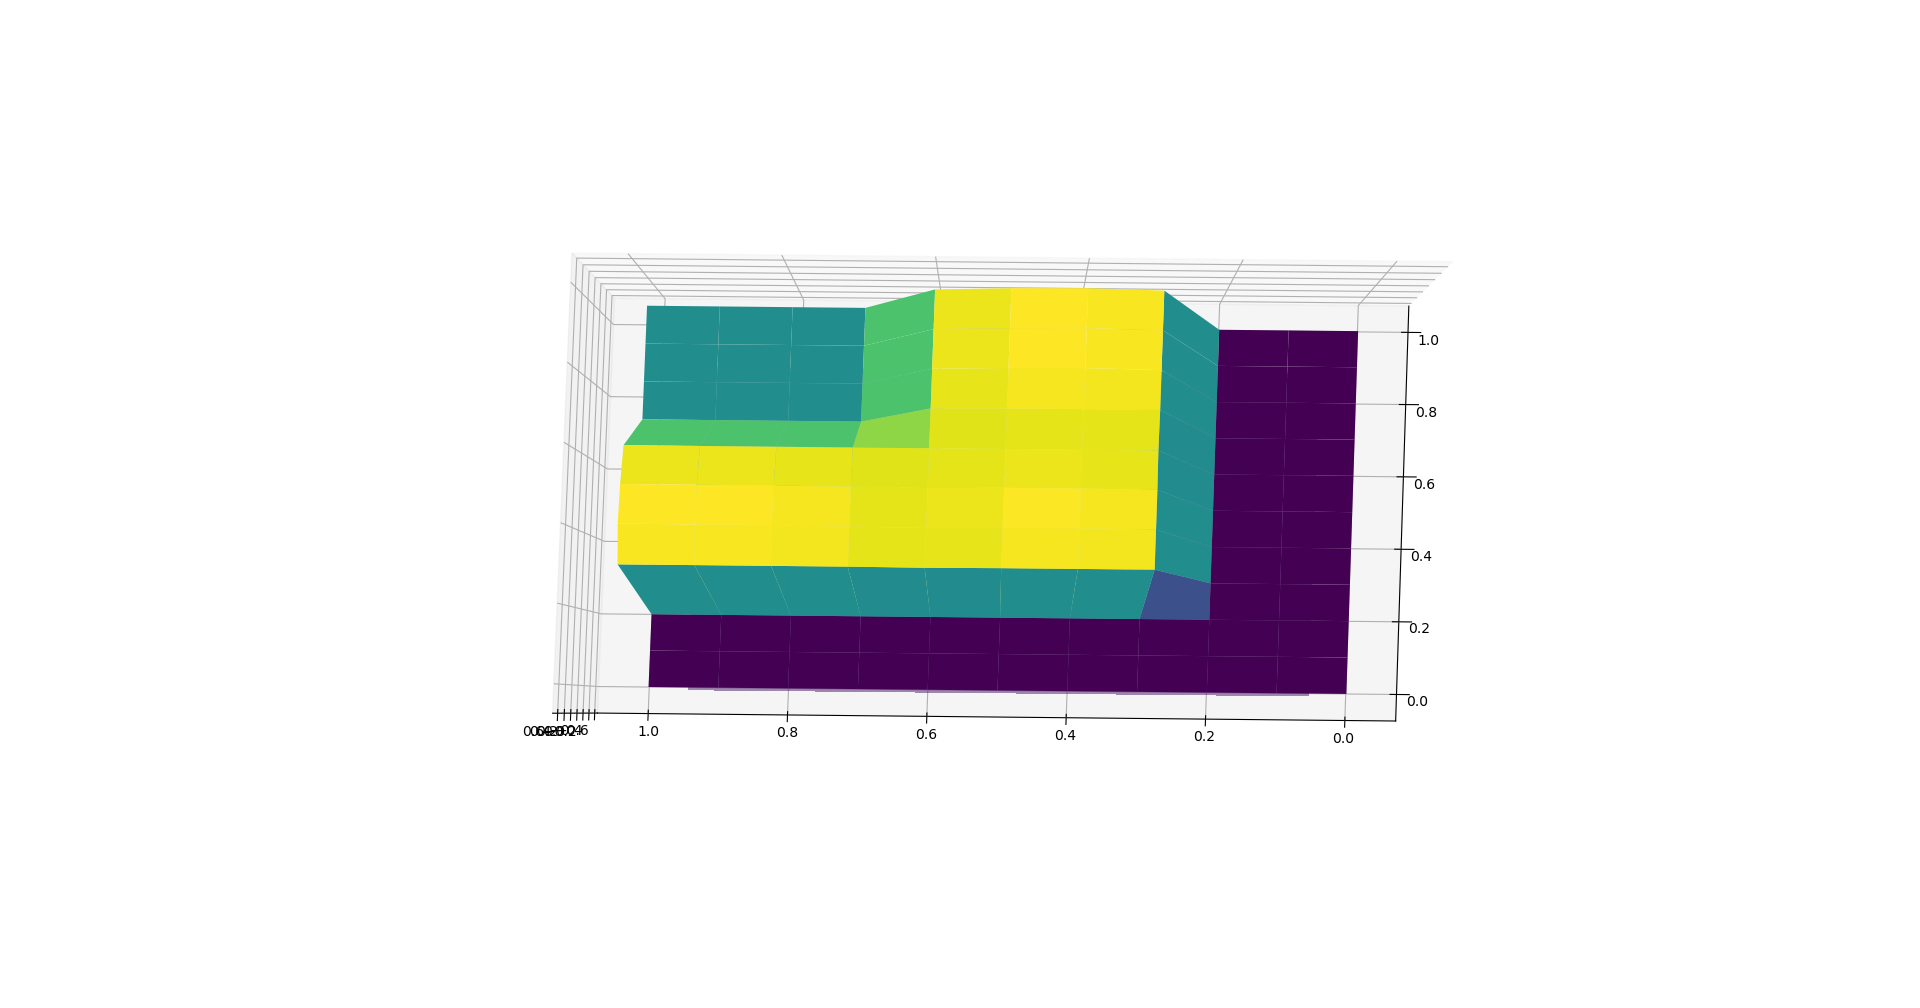
\includegraphics[width = 1\textwidth]{Imagens/Surface_Control2.png}
	 \caption{superfície de controle vista de cima }
	 \label{surface_control2}
\end{figure}


\section{estratégia de treinamento}
O aprendizado por reforço é uma busca por tentativa e erro \cite{sutton2018reinforcement}, ou seja dependendo da complexidade do problema o custo computacional fica bastante elevado. Para mitigar um pouco desse custo foi utilizado uma técnica chamada aprendizagem por demonstração, nela um professor demonstra uma política que é gravada e apresentada ao agente. O objetivo dessa estratégia é dar um conhecimento base ao robô que seria refinado a medida que ele interagisse com o ambiente. Então a estratégia de treinamento ficou:
\begin{itemize}
	\item robô aprende a única demonstração feita 
	\item robô fica em contado com o ambiente simples \ref{scene_1} até melhorar a política demonstrada 
	\item robô fica em contado com o ambiente de validação \ref{scene_2} para mensurar a política aprendida e caso fique tempo o suficiente, refina ainda mais a política aprendida na cena simples \ref{scene_1}. 
\end{itemize}
A cada duzentos movimentos do robô a simulação era reiniciada.

\chapter{Desenvolvimento e Resultados}
Para avaliar o sistema foi feito uma avaliação visual do robô e gráficos da recompensa por movimento do robô. A avaliação visual é verificado se algum momento o robô colide com a parede e pode-se encontrar os vídeos dessa avaliação abaixo:  
\begin{itemize}
 \item \textbf{Primeiro vídeo} \href{https://www.youtube.com/watch?v=DLh3mFDmg-4}{link primeiro vídeo}
 \item \textbf{Segundo vídeo} \href{https://www.youtube.com/watch?v=MQMNd3tqTlU}{link segundo vídeo}
 \item \textbf{Terceiro vídeo} \href{https://www.youtube.com/watch?v=5zjPKKYeF10}{link terceiro vídeo}
 \end{itemize}

nó primeiro vídeo é mostrado desempenho do robô com apenas o conhecimento base, ou seja treinado com a única demonstração. podemos observar que o robô aprendeu que tem que desviar da parede, ele vai chegando perto e bate na parede e sua função de recompensa por movimento reflete esse comportamento \ref{badRewardStep1}.
O segundo vídeo é mostrado o desempenho do robô após algumas interações no primeiro cenário \ref{scene_1}. Novamente o gráfico da função recompensa reflete o seu comportamento, assim como o terceiro vídeo e o terceiro gráfico \ref{rewardStep2}, no entanto vale lembrar que o segundo cenário possui mais obstáculos logo a recompensa por movimento oscila mais.

\begin{figure}
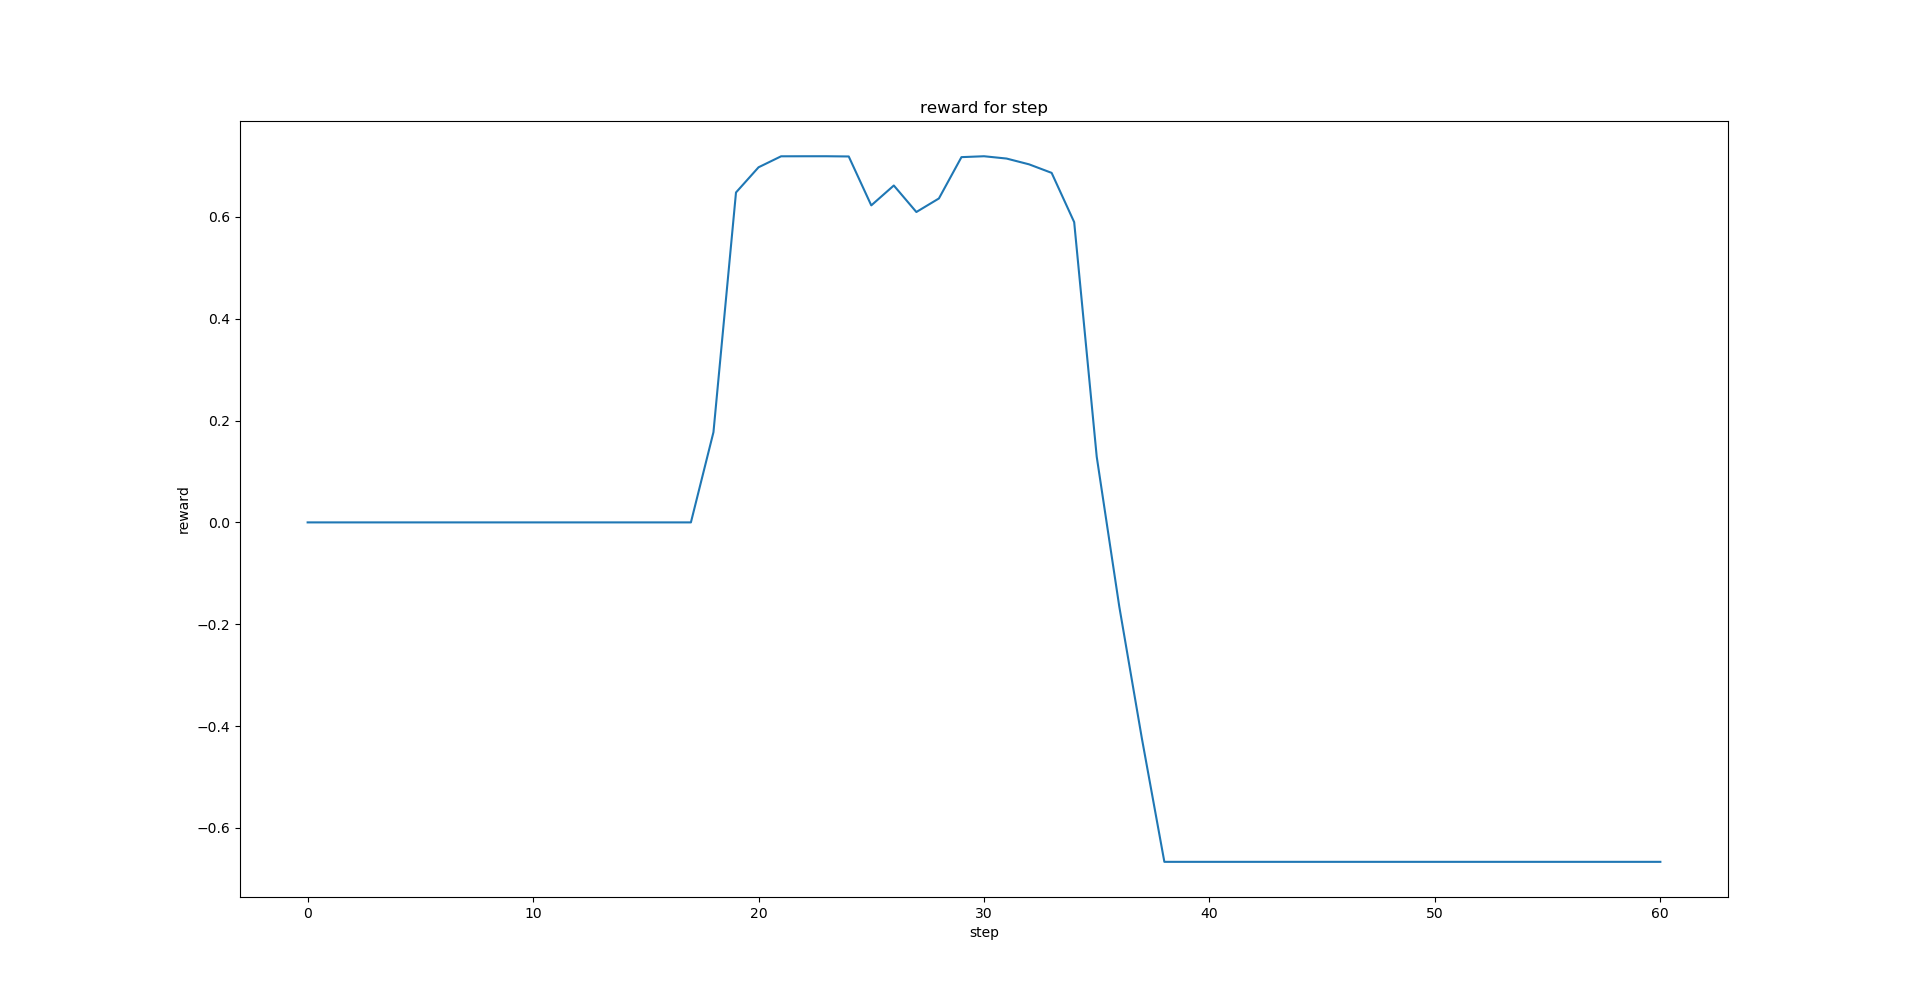
\includegraphics[width = 1\textwidth]{Imagens/badreward_step.png}
	 \caption{gráfico da recompensa do conhecimento base no primeiro cenário \ref{scene_1}}
	 \label{badRewardStep1}

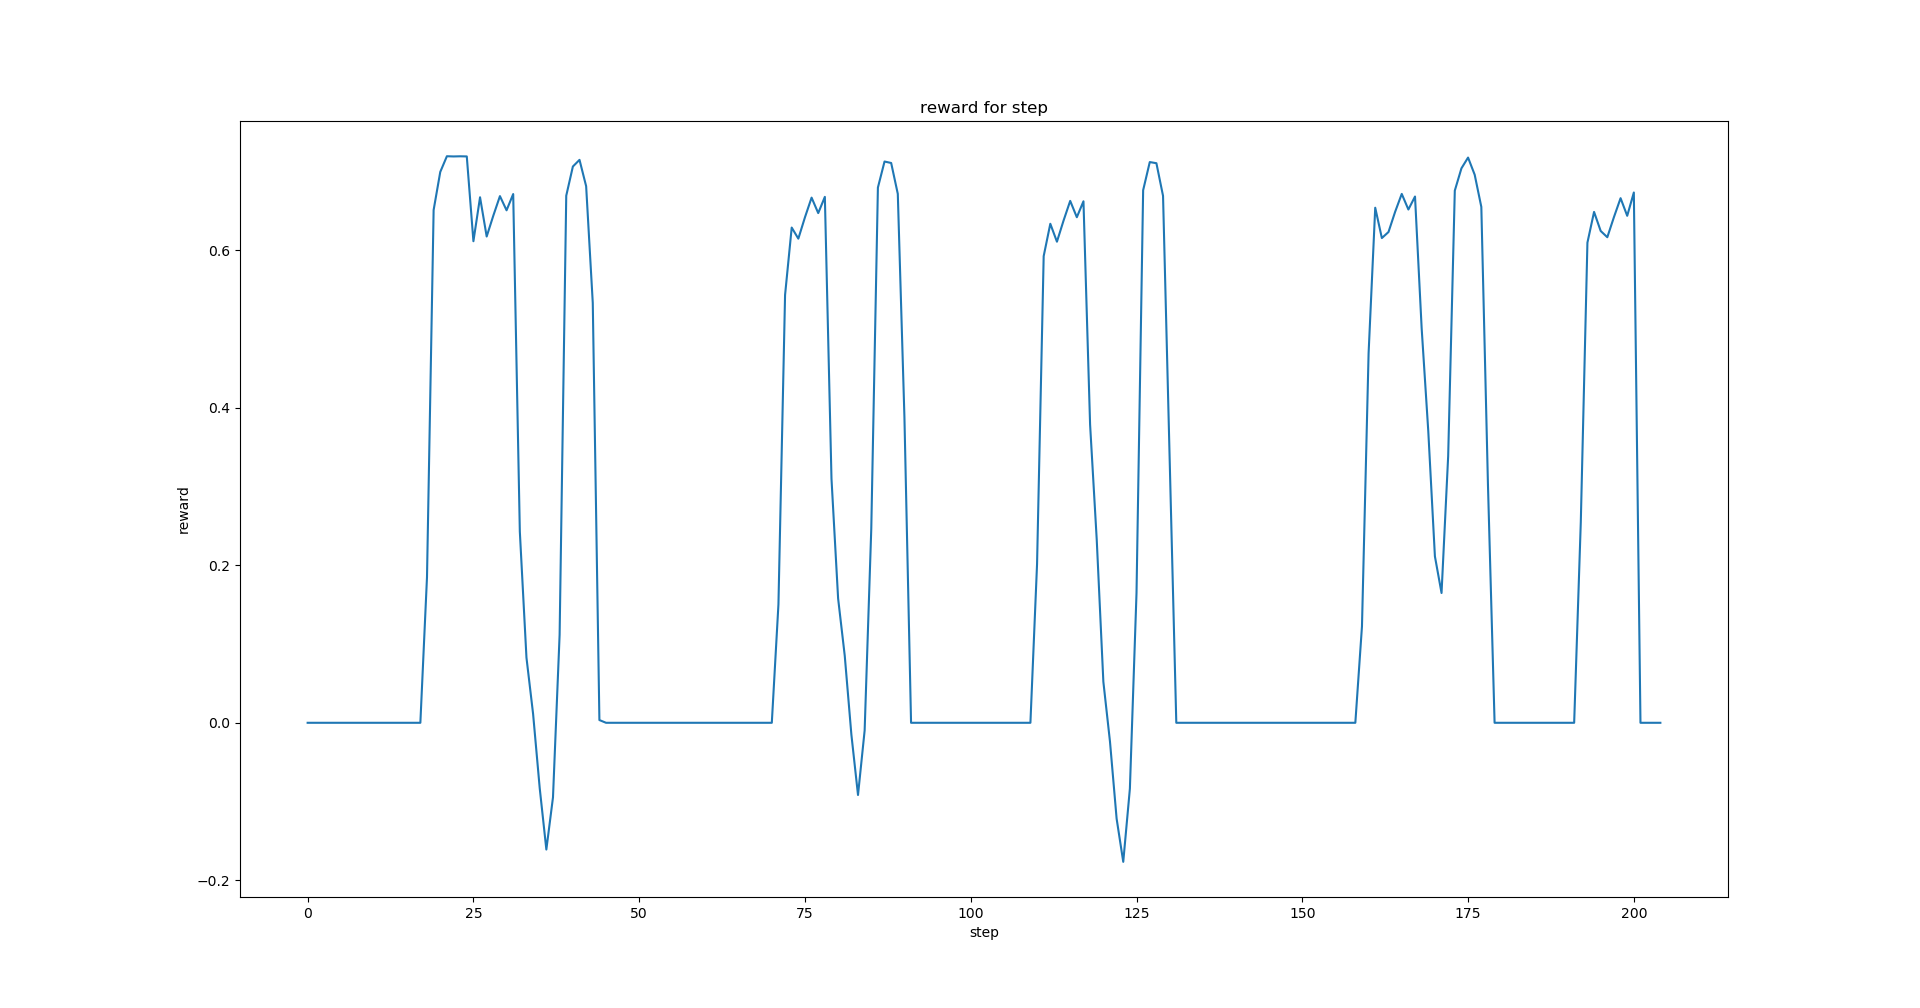
\includegraphics[width = 1\textwidth]{Imagens/reward_step.png}
	 \caption{gráfico da melhor recompensa no primeiro cenário \ref{scene_1}}
	 \label{rewardStep1}

\end{figure}

\begin{figure}
 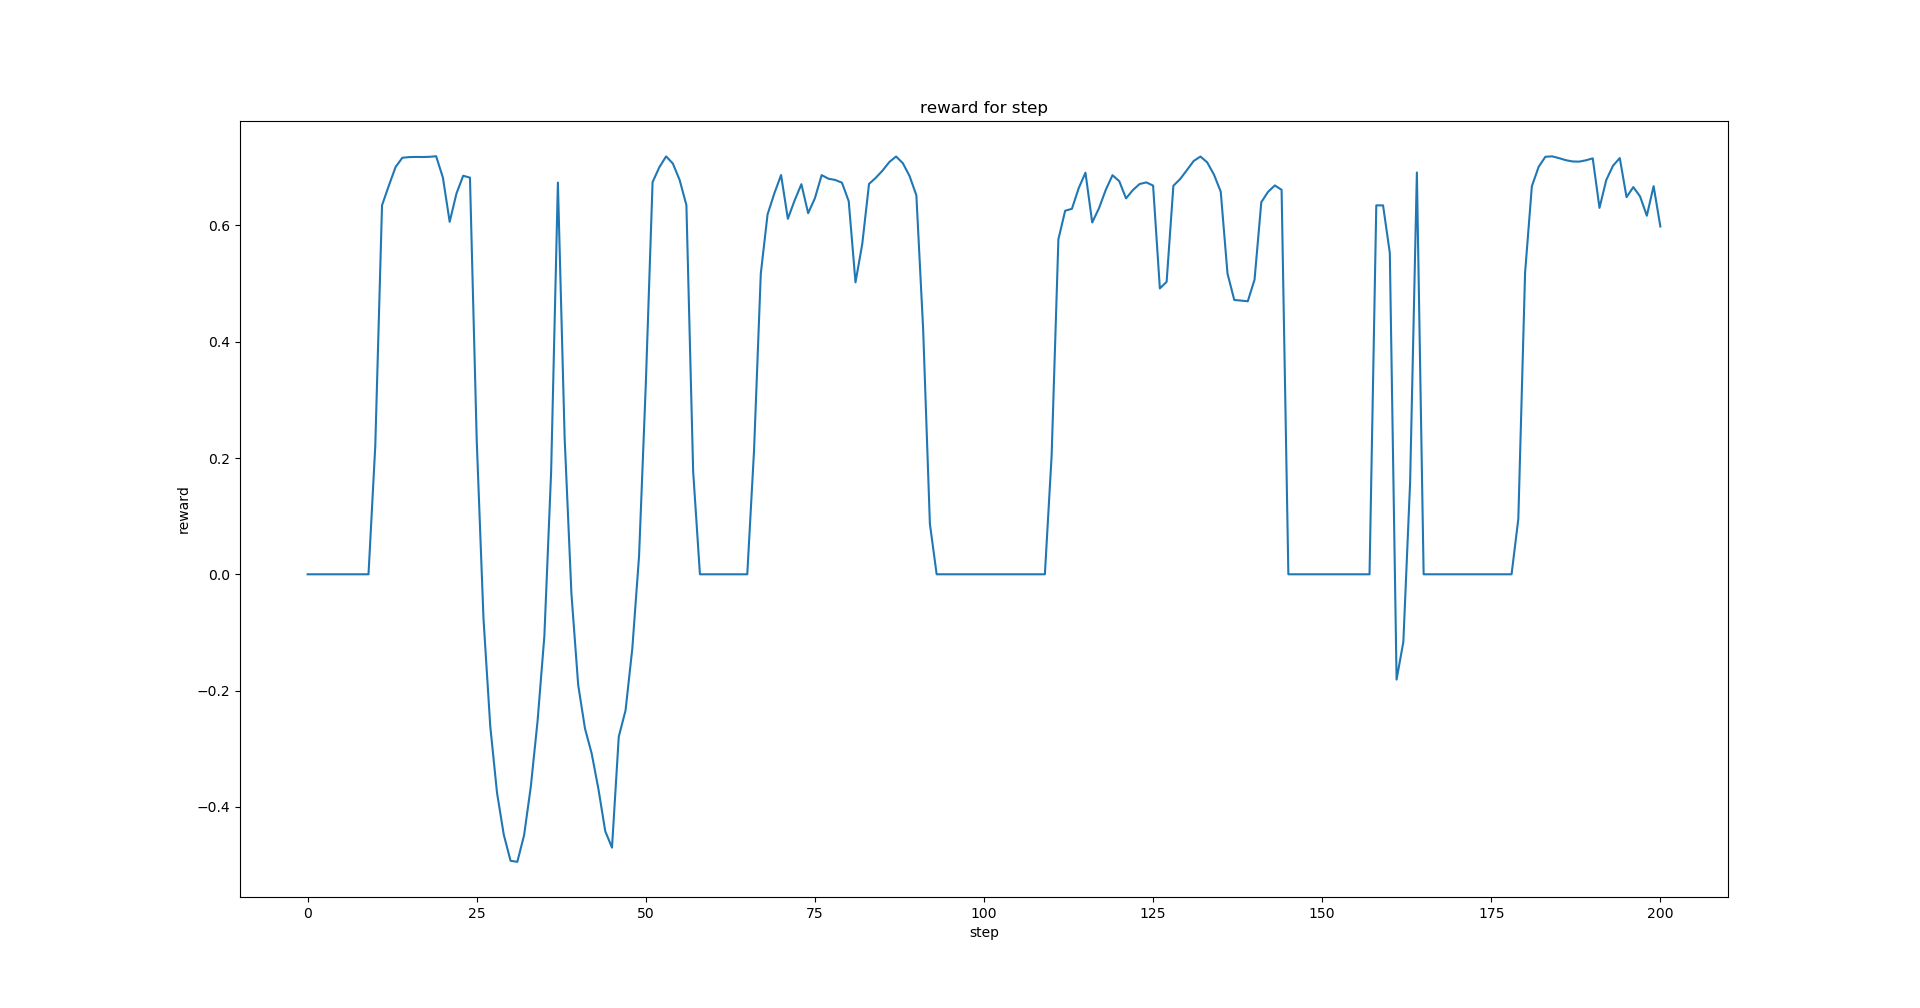
\includegraphics[width = 1\textwidth]{Imagens/reward_step2.png}
	  \caption{gráfico da recompensa no segundo cenário \ref{scene_2}}
	 \label{rewardStep2}
\end{figure}


\chapter{Conclusão}
   A rede convergiu e foi capaz de aprender a desviar de obstáculos. Mostrando que a função de recompensa foi capaz de gerar uma politica ou comportamento satisfatório para o problema. No entanto a função de recompensa foi projetada de modo que recompensa-se o robô a ficar próximo do obstáculo e o robô tende a fugir completamente do obstáculo. Esse comportamento é possivelmente um mínimo local, onde uma das possíveis causas desse fato tenha sido a simplificação do problema, talvez permitindo o agente a se mover para direita e com isso aumentar o número de sensores é possível que o robô consiga sair desse mínimo e consiga melhores resultados 
    
%\bibliographystyle{abnt-alf}
\bibliography{referencias}
    Procure citar todas as referências utilizadas no projeto.

\end{document}